\chapter{Data Understanding: Analysis of the DAM Source Document}
\label{ch:datasource}
\minitoc

\section*{Introduction}
\addcontentsline{toc}{section}{Introduction}

Most data science projects begin with a structured dataset: rows, columns, typed
fields, a distribution to describe and missing values to count. This one begins with a
PDF. There is no dataset to explore until one has been built, and building it is only
defensible if the document it comes from has first been understood on its own terms.

That is the purpose of this chapter. It does three things. It presents the source
document, its provenance, its four-level hierarchy and the authority notation used in its
tables. It then characterises the content quantitatively, establishing what the processed
subset actually contains: how many activities, carrying how many responsibilities,
distributed across which roles and which authority codes. Finally, it documents the ways
in which automated extraction fails on this particular document, each failure mode
identified by comparing extracted output against the printed page rather than inferred
from theory.

The last of these carries the most weight for what follows. Every parsing rule presented
in Chapter~\ref{ch:pipeline} exists to resolve a specific defect catalogued here. Reading
the two chapters in sequence is intended to make the pipeline legible as a response to
evidence rather than as a set of arbitrary engineering choices.

\section{Source Document Presentation}

Before any extraction rule can be justified, the document itself has to be described: where
it comes from, how it is organised, and what notation it uses to record an authority
decision. Every later chapter refers back to the vocabulary established here.

\subsection{Source and Context}

The dataset analyzed in this study comes from the African Development Bank Group’s Delegation of Authority Matrix, which is an internal governance document of more than two hundred and fifty pages distributed in the form of a PDF file. It is not a published research dataset and has no accompanying schema, documentation, or machine-readable export. The DAM has been specifically made to be read by the AFDB staff members. Subsequently, a specific data extraction method needed to be used in order to turn the DAM into a knowledge base. 
At the beginning of the project, work was scoped to a sixty-six pages subset, focusing only on two chapters, as per requested by the client. This initial export was later on replaced by a seventy-nine pages document for two main reasons:
First, the larger file includes the glossary, the abbreviations list, and the authority-code legend, all of which the system needs as reference data rather than as content to be parsed. Second, It contains a full chapter excluded by the initial scope, that is relevant to the proper execution of this project. That chapter was brought into scope once its table structure was examined and found to be compatible with the same parsing approach, at the cost of one substantial new class of layout problem described in Section~\ref{sec:splitrows}.

\subsection{Hierarchical Structure of the Document}

The DAM is structured according to a four-level hierarchy. Thus, the accurate reconstruction of this architectural framework represented a pivotal phase of the study.
At the highest level, “chapters” categorize the AFDB’s activities into broad operational domains. Chapters are further subdivided into processes. These processes are identified by rounded numerical codes (e.g., 2.510) which group related activities. Processes then encompass individual tasks, designated by sequential numbers (e.g., 2.513) and certain tasks decompose further into child tasks, identified by a three-part numerical notation (e.g., 1.117.2). Finally, a small yet important subset of entries consists of threshold variants: sub-items keyed by monetary band rather than sequence number, delegating approval authority based on financial magnitude.

\subsection{Table Layout and the Authority Notation}

Content is presented as wide tables. The leftmost columns carry the activity identifier and its title. The remaining columns each match to an organisational role, and their headers are rotated vertically so that long role names fit within the available width. 
Each cell at the intersection of an activity and a role carries an authority code, or nothing at all if that role has no part in that activity. Alongside the codes, superscript digits refer to footnotes printed at the bottom of the page, qualifying the responsibility with conditions such as delegation limits or specific circumstances.
Two properties of this presentation create most of the difficulty. First, the codes are short, so distinguishing a code from a footnote marker relies on their positions in their respective cells rather than length. Second, the association between a code and a role is purely positional, established by horizontal alignment between a cell and a header printed sideways somewhere above it.

\section{Exploratory Analysis of the Document}

With the document's structure and notation established, the question becomes what the
processed subset actually contains once parsed, from overall node counts down to the
specific record types, roles, and edge cases that shape what the system can and cannot be
asked.

\subsection{Global Overview and Node Distribution}

Once parsed and validated, the seventy-nine-page subset yields 327 nodes, distributed across the four hierarchy levels as shown in Table~\ref{tab:nodedist}. These records carry 1,776 individual responsibility entries, each one an assertion that a named role holds a specific authority code over a specific activity.

\begin{longtable}{|p{0.30\textwidth}|p{0.14\textwidth}|p{0.44\textwidth}|}
\caption{Distribution of node types across the processed subset.}\label{tab:nodedist}\\
\hline
\rowcolor{myblue}\textcolor{white}{\textbf{Node type}} & \textcolor{white}{\textbf{Count}} & \textcolor{white}{\textbf{Description}} \\
\hline
\endfirsthead
\hline
\rowcolor{myblue}\textcolor{white}{\textbf{Node type}} & \textcolor{white}{\textbf{Count}} & \textcolor{white}{\textbf{Description}} \\
\hline
\endhead
Chapter & 3 & Top-level domains of Bank activity covered by the processed subset. \\ \hline
Process & 35 & Groups of related activities within a chapter. \\ \hline
Task & 138 & Individual activities, the level most questions are about. \\ \hline
Child task & 102 & Sub-activities of a task. \\ \hline
Threshold variant & 49 & Variants of a task keyed by a monetary threshold band. \\ \hline
\textbf{Total} & \textbf{327} & \\ \hline
\end{longtable}


Following the table above, we can see that even with only three chapters, we can see that they produce 35 processes, and therefore the processes have 240 tasks, of which 102 are child tasks and sub-activities. The proportion of threshold variants is higher than an outside reader might expect, and it reflects something about how the AFDB delegates authority. Approval rights are frequently banded by amount. Thus, a single named activity can carry three or four different approvers depending on the sum at stake. A system that treated each activity as having one answer would be wrong for roughly fifteen percent of the document.

\subsection{Authority Code Distribution}

Across the 1,776 responsibility entries, the codes are not evenly distributed. Informed markers and check-and-verify obligations are considerably more common than approvals which is unsurprising. As a matter of fact, a single approval is usually surrounded by several roles that are set to verify the work beforehand and numerous more that must be notified afterwards.\\[0.3cm]
This statement can be illustrated by an example: a user happens to generate a query asking about who approves a certain activity and the system responds to the said query with strictly the approver. The response given by the system does not include the prerequisite steps and/or subsequent actions that need to be fulfilled in order to transfer approval. In other words, the system is considered to have partially answered the query and has omitted the mandatory obligations attached to it. This observation leads to understanding the need for requirement FR4, and the behaviour it specifies is further explained in Chapter 4.

\subsection{Role and Actor Analysis}

The document names 131 distinct roles across the processed subset, ranging from country office staff through sector managers, division managers, directors, and vice- presidents, all the way up to the Board. However, role names are long and heavily abbreviated. This issue had led to primarily considering the vertically rotated headers previously mentioned and the abbreviations are not always defined in the document’s own glossary.\\[0.3cm]
That last point produced a small yet visible feature of the finished system. In spite of the fact that some acronyms appear throughout the role names, they remain separately undefined  in the abbreviations pages. As a result, the system is set to maintain a small set of curated aliases for the acronyms that are not defined, avoiding the burden for the user to look for it by themself. Additionally, the system will clearly state when an expansion is drawn from that curated set instead of the glossary provided in the document. This feature provides a more transparent and easily understandable navigation through the system for the user. \\[0.3cm]
Averaged across all 327 records, each activity carries an average of  5.48 responsibility entries. Just under thirty percent of records carry no direct responsibilities at all, which at first looks like an extraction failure and mostly is not. Chapters and processes are organizational containers rather than activities, so they legitimately have none, and a further group of tasks are pure cross-references, discussed below.

\subsection{Threshold Variants and Monetary Bands}

Threshold variants were not part of the initial understanding of the document’s structure. Indeed, these threshold variants were detected during the data extraction process, when rows appeared in the shape of a task’s sub-item while carrying a monetary band instead of a sequential number. 
In order to correctly identify the task, the threshold variants needed to be acknowledged as a separate level of a task rather than forcing them into the child-task category. This distinction is also explained by the different natures of both categories : on one hand, a child task is a component of a task. On the other hand, a threshold variant is an alternative to its siblings. 

\subsection{Cross-References and Redirects}

A few entries in the DAM document record no responsibilities but instead have references to other parts of the document. These references come in two ways. One way involves a list of explicit references that are presented as “See DAM 16.100, 16.200,” and similar forms. The second way is by way of a range of references, which are said as “Refer to Activities 2.114 - 2.117 in Section 2.” This needs to be further elaborated into a list of all identifiers in the range and not just the two endpoints.
Fourteen references like these were found in the analyzed set of data. When one sees this kind of statement, he or she will go through the pages referred to and continue analysis. The system is expected to follow the references because when someone asks for activity 1.117.2 and receives the answer that it has no responsibility listed, that answer is accurate but practically useless.

\subsection{Consolidated View}

In combination, the exploratory analysis reveals some conditions for all further work done on the document. The document has a hierarchical structure; nevertheless, it cannot be derived from identifiers’ names. It is a positionally meaningful structure, and is coded by the association of cells with vertically turned headers. Quite a significant number of rows in this document represent not activities but pointers or threshold options. Furthermore, most responsibilities listed here are the ones that would be considered secondary by a naïve question answering system.

\section{Extraction Quality Assessment}


This section highlights the inconsistencies found when the document is processed automatically. Every bug described below was identified through comparison of the output produced with the corresponding printed page it was taken from. Such a method takes more time than verification of correct code execution, but it is the only way to find such problems because any failure here results in totally believable output until it is compared with the source. 

\subsection{Text Layer Inspection}

PDF is a page description format. It contains the information about which glyph is drawn at each particular coordinate in a particular font and size. It does not contain any information about the semantic meaning of the group of these glyphs. Libraries like pdfplumber extract characters and words along with their positions. However, all structural properties have to be restored from the geometrical one because it is not done by the library. In the file "row" is not "row". It is the set of words having close enough vertical positions. How close enough is not defined anywhere and can be determined empirically only.

\begin{figure}[htbp]
\centering
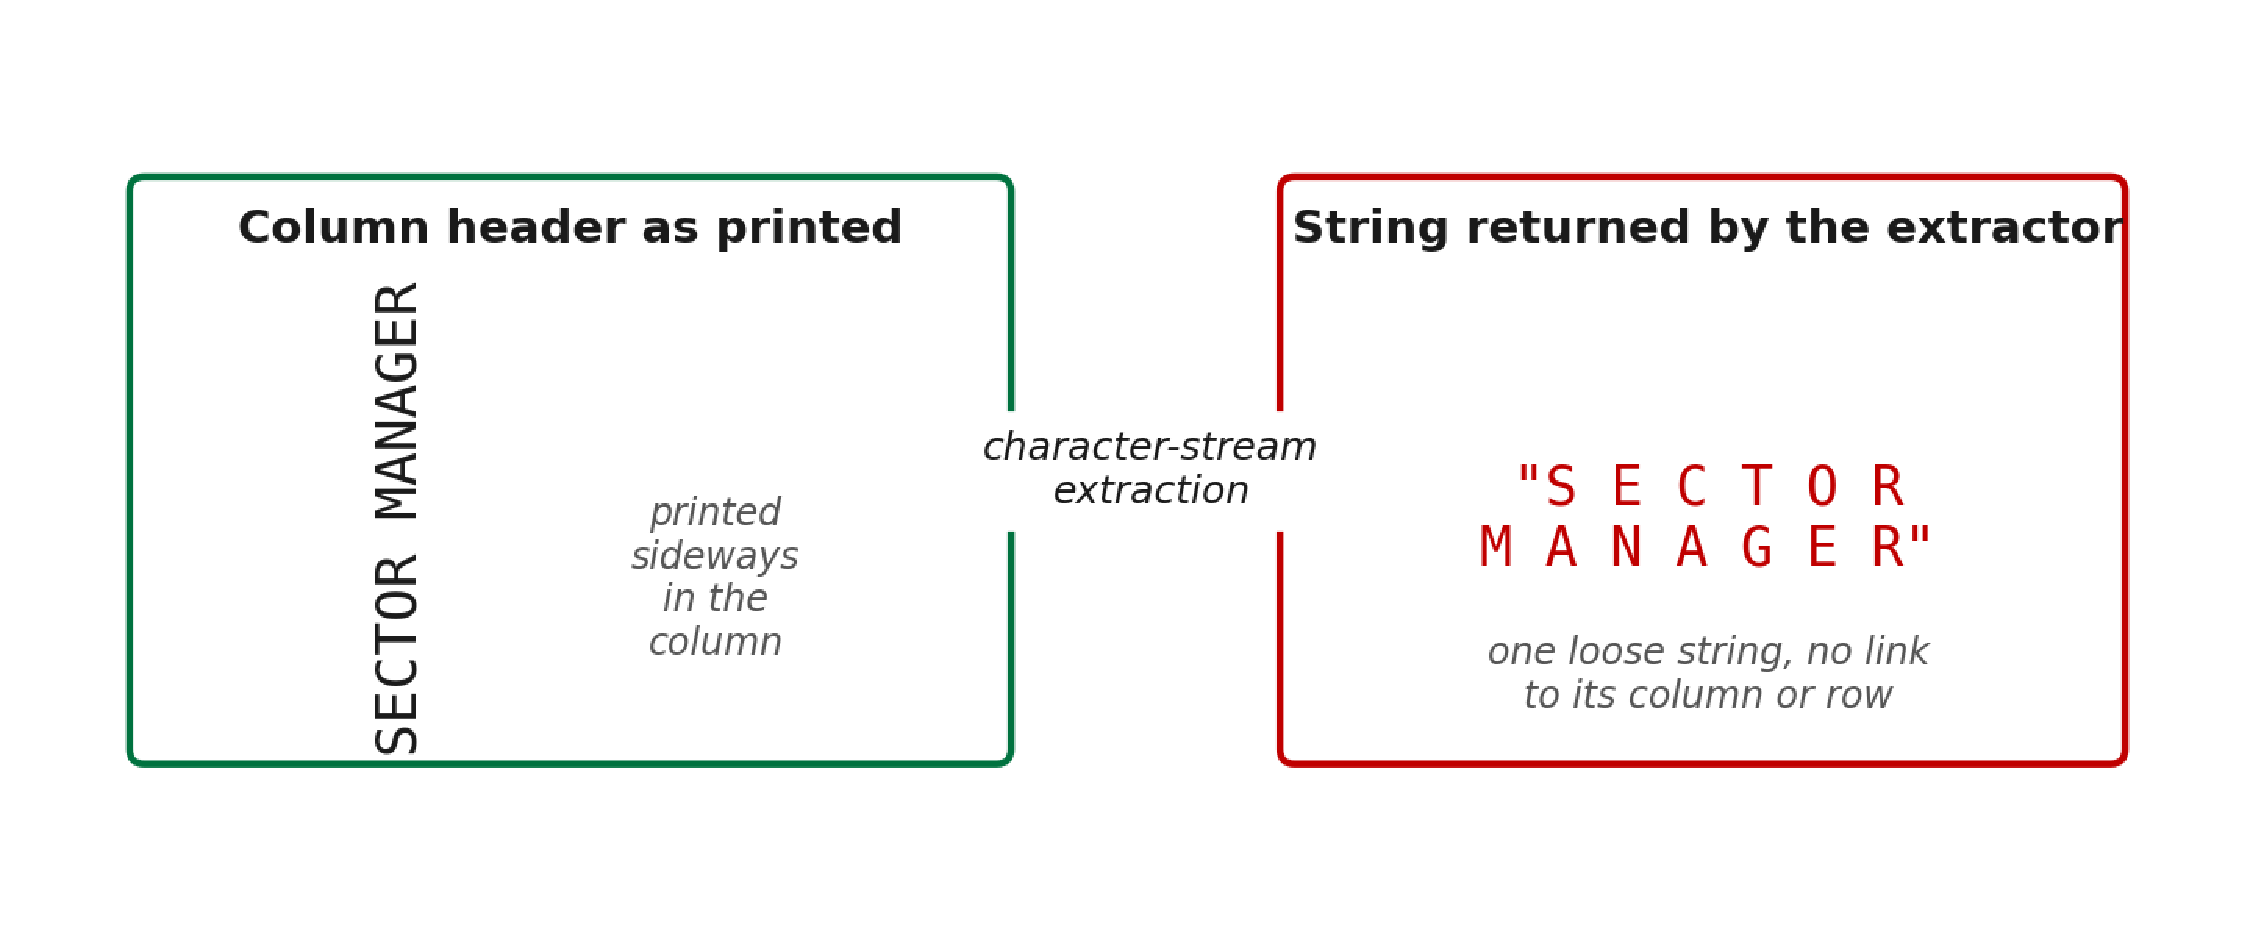
\includegraphics[width=0.92\textwidth]{figures/fig2_rotated_headers.pdf}
\caption{Column headers as printed, rotated through ninety degrees, beside the text an
extractor returns for the same region. The header row is not recoverable as a table header.}
\label{fig:rotatedheaders}
\end{figure}

\subsection{Rotated Column Headers}

The headers and the text an extractor returns for them are shown side by side in Figure~\ref{fig:rotatedheaders}.

Headers for roles are printed vertically. When the standard word extraction is used, they appear just as plain words with usual coordinates, which means that nothing is known about their rotation and the horizontal position of the word corresponds to the narrow strip of the rotated text rather than the whole column underneath it. Therefore, in order to attribute any code to some role, header words have to be clustered by their horizontal position and each cell should be associated with the nearest header cluster. The problem occurred somewhere in the middle of the document: some pages have headers only once and the table continues further without them. These pages have codes but no headers, so attribution fails unless the last seen headers are used instead.

\subsection{Fused Footnote Digits and Authority Codes}

Figure~\ref{fig:fusedfootnote} shows a code and its footnote marker as printed, alongside the fused token that results when the size difference between them is disregarded.

The footnote markers are encoded as the superscripts adjacent to the authority code. After extraction, if the code A and the footnote 3 occur, the string “A3” is produced, which visually cannot be distinguished from the correct level-bearing code “A3.” The distinction can be made only on the basis of the vertical offset of the digits from the baseline and the difference in font sizes between the digit and the letter. Superscripts appear at higher offsets and in smaller fonts, and the rule was established experimentally based on real-life examples of characters, not on intuitive assumptions, since the offsets are small, and an intuitively guessed threshold would result in a significant number of misclassifications.
Another flaw impacted the informed marker. Since the marker consisted of the parenthesized character i, it could be detected by the string “(i)” in the text. However, on a real-life page, this marker consists of five separate characters, so nothing matched. Before this problem was discovered, of the 276 records in an early version of the extraction, 174 included the informed marker inside the printed document that had no impact on the extracted data. This flaw remained undetected until the output involved record comparison with the page. It can be explained by the fact that there is an additional Authority code when flattened produces the same string “I”.

\begin{figure}[htbp]
\centering
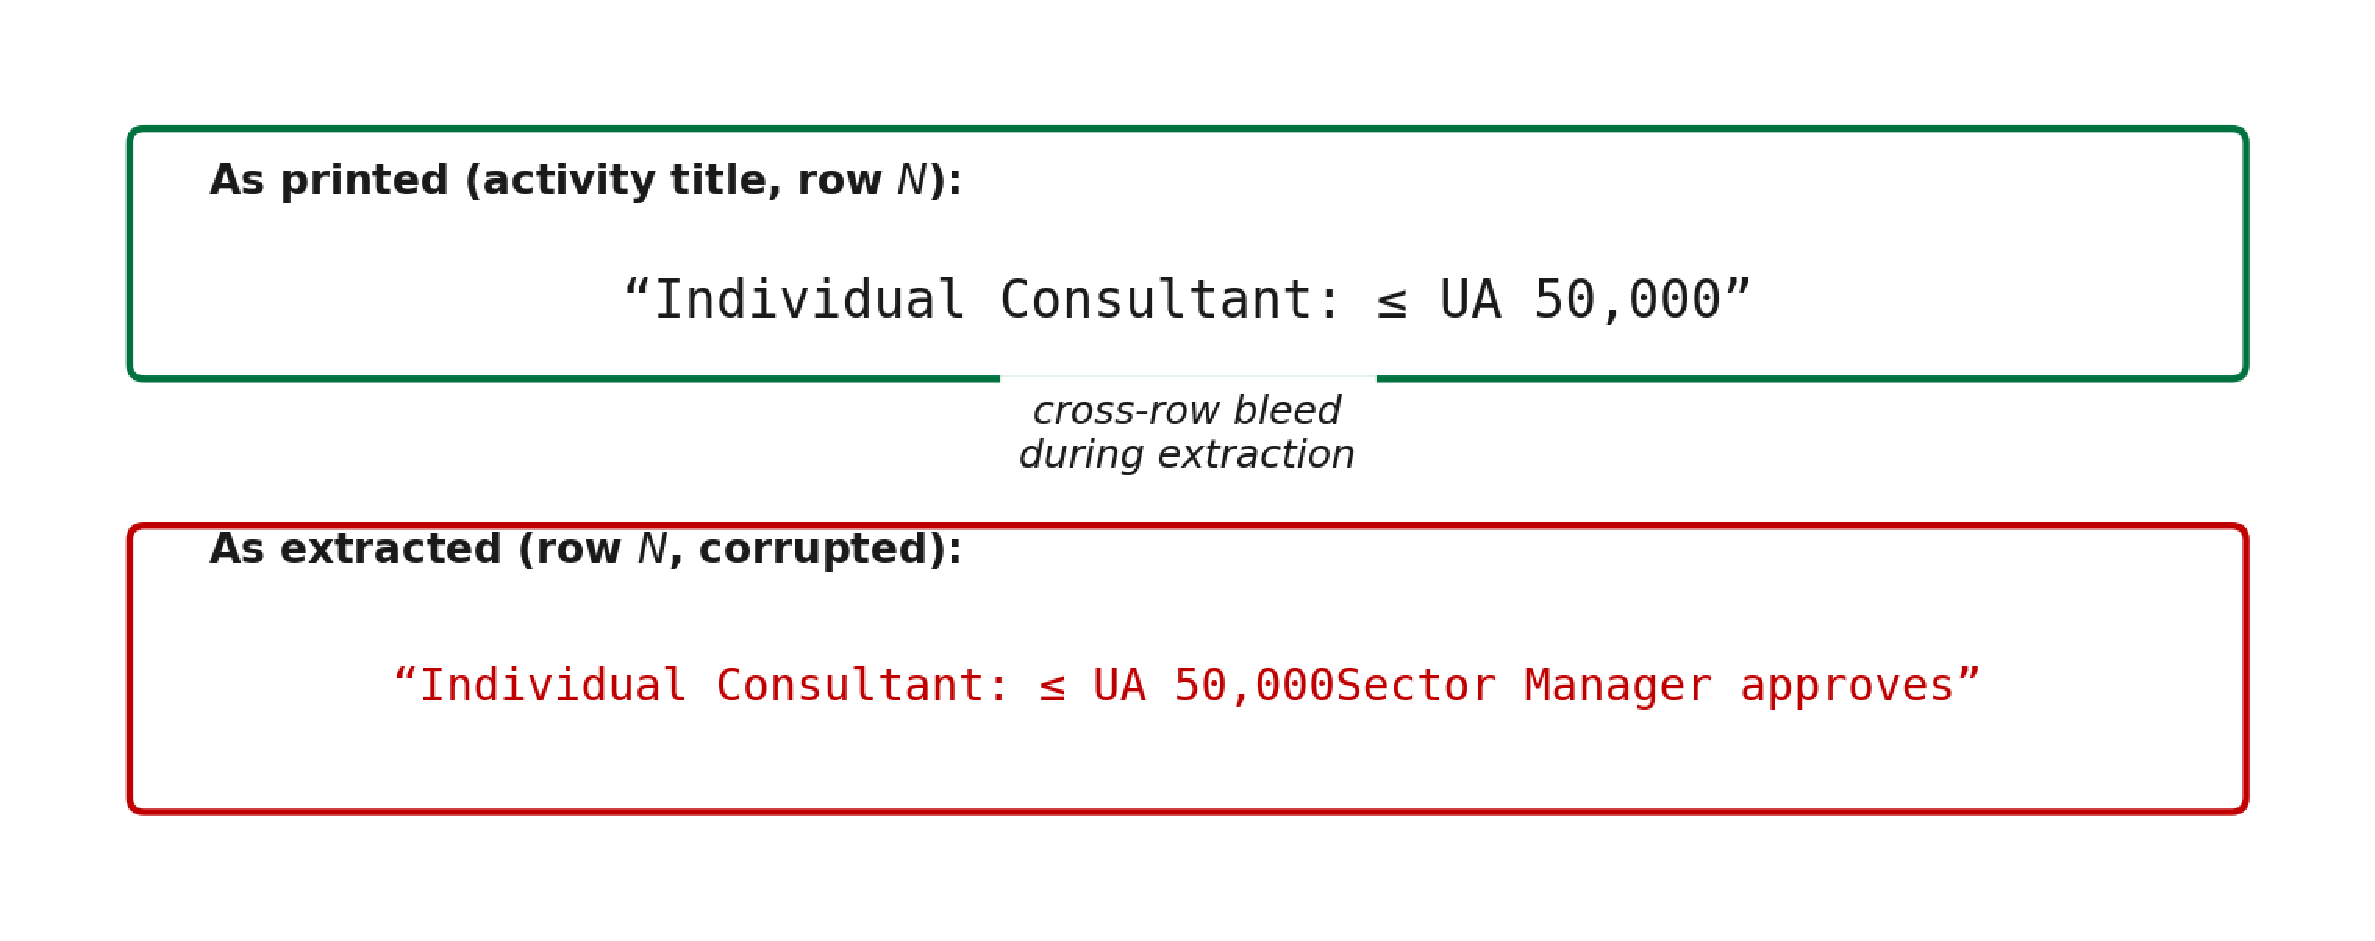
\includegraphics[width=0.92\textwidth]{figures/fig2_title_corruption.pdf}
\caption{An activity title as printed, and the corrupted string produced when text from an
adjacent row bleeds into it during extraction.}
\label{fig:titlecorruption}
\end{figure}

\subsection{Cross-Row Text Bleeding and Title Corruption}

Figure~\ref{fig:titlecorruption} pairs a printed title with the corrupted string extracted for the same activity.

The activity titles can consist of several lines, so a line of the title of one activity can be closer to the row of another activity in a dense table. In such situations, the title is associated with the wrong activity. Therefore, both activities are valid by themselves : one of them contains an overly short title, while the other is overly long, and there is nothing indicating that an error has occurred.
At its worst, the problem occurred in roughly one-quarter of the records generated by a preliminary version of the parser. This was resolved through the use of a system where in title attachment depended on the parse state rather than just proximity, utilizing the following three criteria: (1) is there currently an open task, (2) does the open task's text end in a period, and (3) does the line have authority codes when the open task already has them? After implementing these rules, the sole outstanding case occurred in the entire set of records for activity 2.222.1, a documented exception rather than an automatic acceptance.

\subsection{Split Rows in the Non-Sovereign Operations Chapter}
\label{sec:splitrows}

With the introduction of the Non-Sovereign Operations chapter, as well as the need to define scope after the initial parsing of the text, a layout exception was introduced wherein a single logical row was sometimes laid out as two separate rows, with the authority codes appearing a bit below the activity text. The first attempt at correction consisted of simply merging any two vertically contiguous bands separated by less than some tolerance level. A check done before implementation showed 1,614 candidates mergers in the document, but many of them were incorrect and would have merged unrelated activities. This general solution was therefore dismissed, and a more limited one adopted whereby only a band containing nothing other than authority codes was merged, a strong indicator that it was part of the row above it.

\begin{figure}[htbp]
\centering
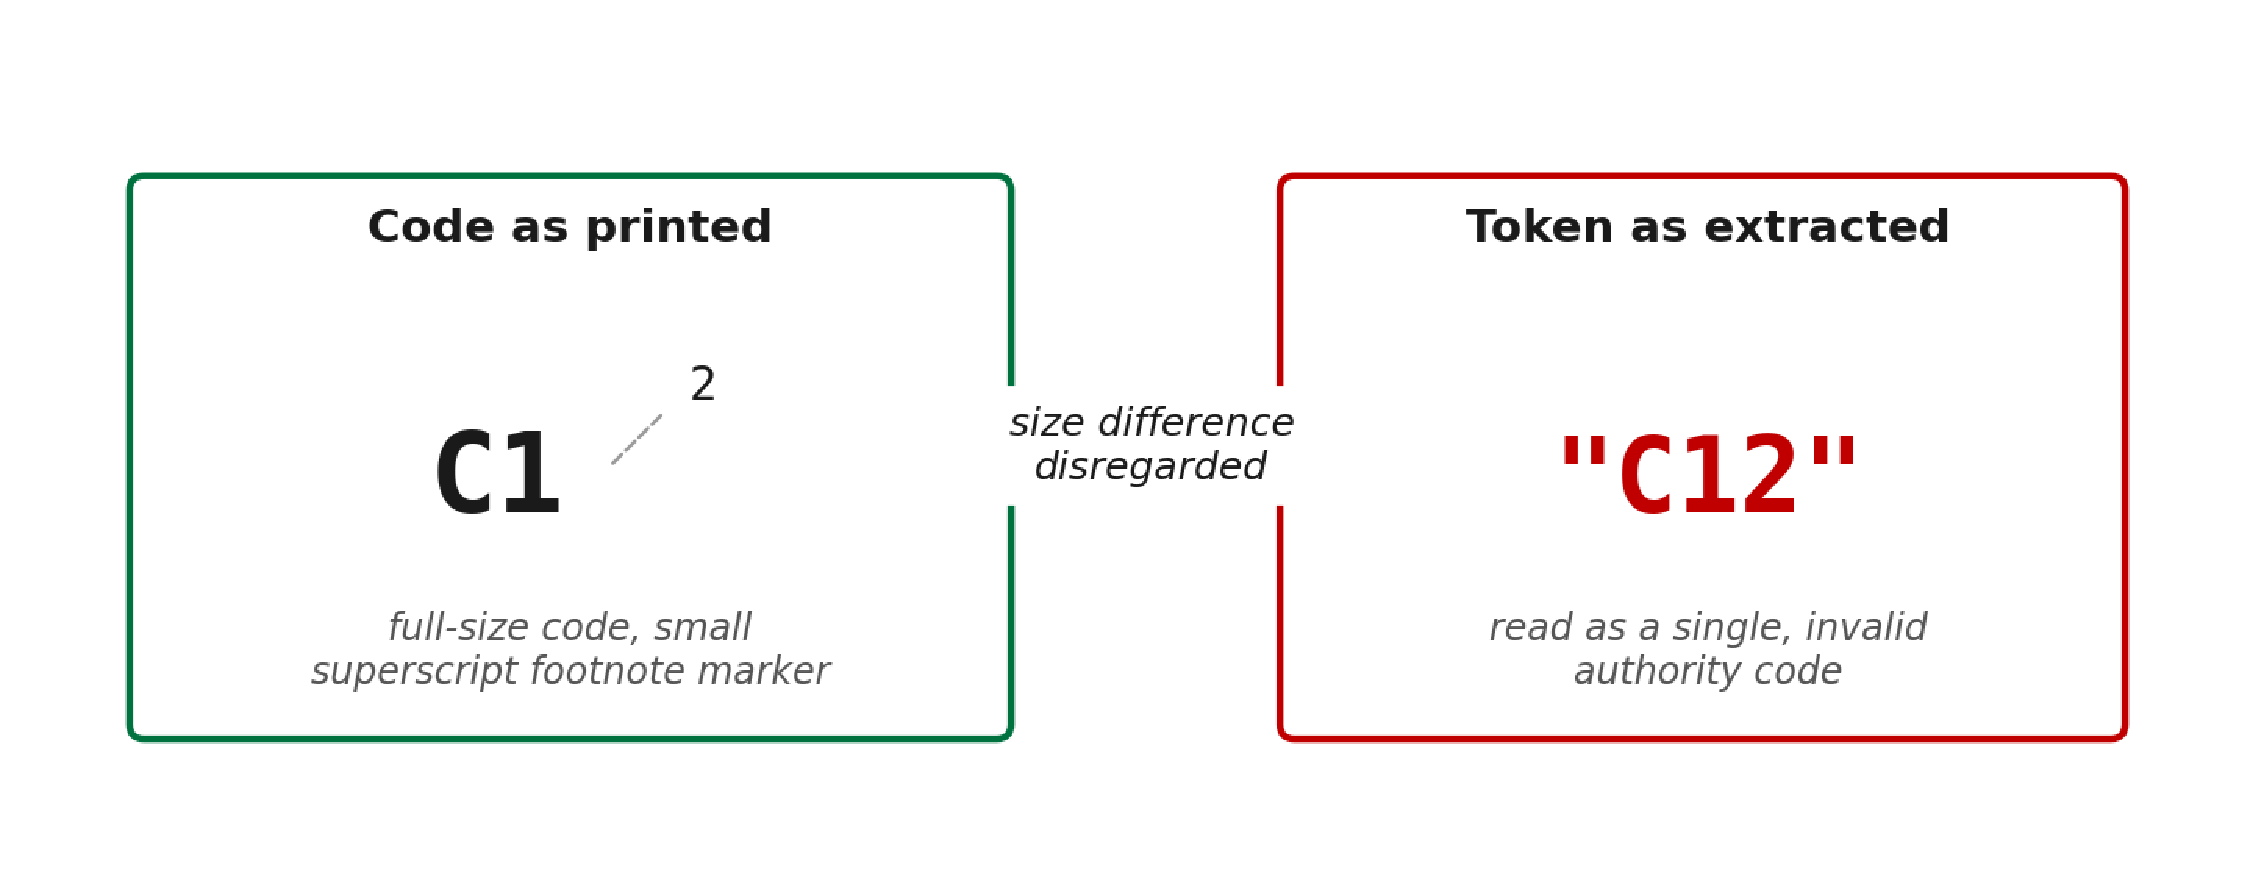
\includegraphics[width=0.78\textwidth]{figures/fig2_fused_footnote.pdf}
\caption{An authority code printed beside a superscript footnote marker, and the fused token
produced when the size difference between them is disregarded.}
\label{fig:fusedfootnote}
\end{figure}

\subsection{Consolidated Data Issues Summary}

Table~\ref{tab:issues} consolidates the defects described above, each paired with the stage of the pipeline that addresses it.

\begin{longtable}{|p{0.24\textwidth}|p{0.30\textwidth}|p{0.34\textwidth}|}
\caption{Consolidated summary of extraction issues found in the source document.}\label{tab:issues}\\
\hline
\rowcolor{myblue}\textcolor{white}{\textbf{Issue}} & \textcolor{white}{\textbf{Effect if unhandled}} & \textcolor{white}{\textbf{Resolution}} \\
\hline
\endfirsthead
\hline
\rowcolor{myblue}\textcolor{white}{\textbf{Issue}} & \textcolor{white}{\textbf{Effect if unhandled}} & \textcolor{white}{\textbf{Resolution}} \\
\hline
\endhead
Rotated column headers & Codes cannot be attributed to roles. & Cluster header text by horizontal position; carry the header set forward across continuation pages. \\ \hline
Missing headers on continuation pages & Whole pages of responsibilities lost. & Reuse the last seen header set until a new one appears. \\ \hline
Footnote digits fused with codes & Codes misread; footnote qualifications lost. & Separate by measured vertical offset and font size of the character. \\ \hline
Informed marker not matched & Informed parties absent from the majority of records. & Match the marker as the separate characters it is actually rendered as. \\ \hline
Title bleeding across rows & Titles attached to the wrong activity; free-text search degraded. & Conditional attachment based on parse state, terminating punctuation, and code presence. \\ \hline
Split rows in the NSO chapter & Responsibilities detached from their activity. & Merge a band only when it consists entirely of authority codes. \\ \hline
Hierarchy from string prefixes & Two of four hierarchy levels silently wrong. & Derive parentage from explicit parent fields and process arithmetic. \\ \hline
Cross-reference rows & Activities reported as having no responsibilities. & Extract references, expand ranges, and follow pointers at query time. \\ \hline
\end{longtable}

\section*{Conclusion}
\addcontentsline{toc}{section}{Conclusion}
DAM can be seen as a well-written document for humans, and as an adversarial artifact for the parser, given that all the structural features that this artifact has can be conveyed using its structure. The problems presented in this chapter do not constitute edge cases. Rather, they together impact all the components in the answer that the parser should provide : the hierarchy, roles, titles, and informed parties. Furthermore, this chapter presents a methodology that can be applied in practice. None of these problems were detected using code inspection or by inferring what the parser was supposed to output. Rather, each problem was detected by collecting the output and comparing it against the corresponding page. This methodology continues in all subsequent parts of this thesis, as discussed in Chapter 3.